\documentclass[A4]{scrartcl}
\usepackage[paper=a4paper,left=10mm,right=10mm,top=25mm,bottom=25mm]{geometry}
\usepackage{graphicx}

%TODO : Klausur-SYT-SS18 nachtragen
\begin{document}
  \addsec{Verständnisfragen}
  Wann liefert die Formel $V(s) = G(s)U(s)$ den richtigen Verlauf der Ausgangsgröße? ?\\
  Antwort:\\\\
  Sie kennen die DGL eines LZI-Systems. Wie können Sie den Frequenzgang des Systems theoretisch berechnen?\\
  Antwort:\\\\
  Wie können Sie den Frequenzgang eines stabilen LZI-Systems experimentell ermitteln?\\
  Antwort:\\\\
  Beweisen Sie mit den Mitteln der Laplace-Transformation, das h(t) das Integral von g(t) ist!\\
  Antwort:\\\\
  Was unterscheidet die gewöhnliche Differenziation von der verallgemeinerten Differenziation?\\
  Antwort:\\\\ 
  
  Bei einem linearen System:\\\\
  $\circ\circ$ist die Ausgangsgröße immer eine lineare Funktion\\
  $\circ\circ$ist die Eingangsgröße immer eine lineare Funktion\\
  $\circ\circ$überlagern sich die Wirkungen der Eingangsgrößen additiv\\
  $\circ\circ$darf keine Totzeit enthalten sein\\

  Bei einem zeitinvarianten System:\\\\
  $\circ\circ$enthält das System keine dynamischen Glieder\\
  $\circ\circ$enthält das System keine nichtlinearen Glieder\\
  $\circ\circ$ist der Ausgang immer konstant\\
  $\circ\circ$enthält das System keine zeitabhängigen Parameter\\

  Bei einem stabilen LZI-System:\\\\
  $\circ\circ$kommt der Ausgang immer zur Ruhe \\
  $\circ\circ$geht die Übergangsfunktion auf Null\\
  $\circ\circ$geht die Impulsantwort auf Null\\
  $\circ\circ$treten keine Schwingungen auf\\

  Wie kann mit Hilfe von g(t) der Systemausgang v(t) prinzipiell nicht berechnet werden:\\\\
  $\circ\circ$mit dem Faltungsintegral \\
  $\circ\circ$mit $v(t) = g(t) \cdot u(t)$\\
  $\circ\circ$mit der Laplacetransformation\\
  $\circ\circ$mit der Fouriertransformation\\

  \newpage
  Die Zustandsraumdarstellung:\\\\
  $\circ\circ$verwendet Matrizen.\\
  $\circ\circ$beruht auf Differentialgleichungen 2. Ordnung\\
  $\circ\circ$ist nicht für Mehrgrößensysteme geeignet\\
  $\circ\circ$arbeitet im Bildbereich der Laplace-Transformation\\


  \addsec{Laplace/Fourier Trafo}
  Gegeben sei folgende Zeitfunktion:\\
  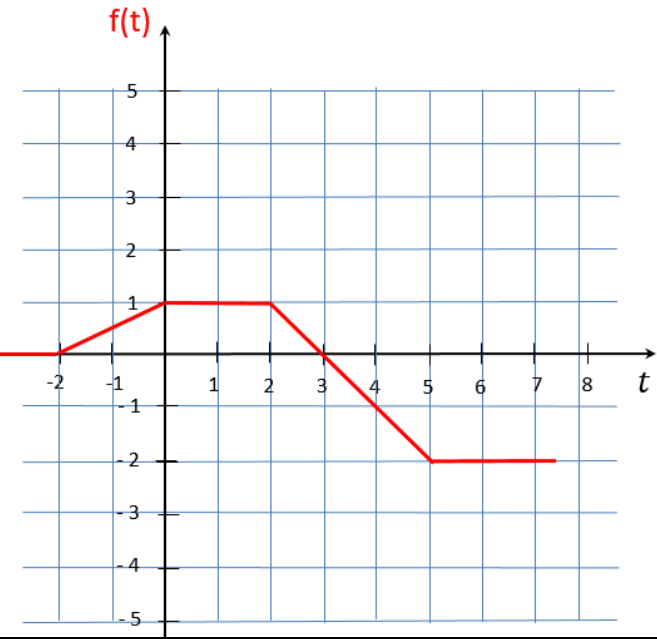
\includegraphics{zeitfunktion1.png}\\
  a) Bestimmen Sie f(t)!\\
  b) Handelt es sich bei f(t) um ein Energiesignal? (Begründung erforderlich)\\
  c) Bestimmen Sie die Laplace-Transformierte F(s) = L{f(t)}!\\
  d) Bestimmen Sie die Laplace-Transformierte der um 3 nach rechts verschobenen Zeitfunktion f(t - 3)!\\
  \newpage
  Gegeben sei folgende Schaltung:\\
  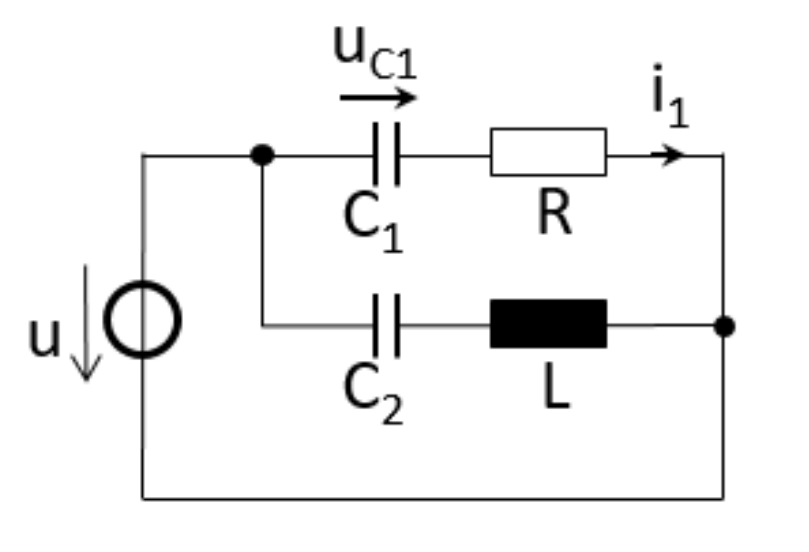
\includegraphics{Schaltung1.png}\\
  a) Bestimmen Sie die Übertragungsfunktion $G(s) = \frac{I_1(s)}{U(s)}$!\\
  b) Bestimmen Sie die zugehörige DGL!\\
  c) Bestimmen Sie $g(t)$!\\
  \newpage
  Gegeben ist die Übertragungsfunktion $G(s) = \frac{10}{(s+0,5)(s+4)}$\\
  a) Ist das System stabil (Begründung erforderlich)!\\
  b) Berechnen Sie die Einschwingzeit von h(t)!\\
  c) Mit welchem Faktor wird für großes t die Amplitude der Eingangsschwingung $u(t) = sin(10t)$ verstärkt!\\
  d) Der Eingang ist nun $u(t) = (1-e^{-t})\sigma(t)$. Berechnen Sie U(s)!\\
  e) Bestimmen Sie v(t) für den Eingang aus d)! (Anfangswerte sind 0)!\\
  \newpage
  Gegeben sei folgende Zeitfunktion f(t):\\
  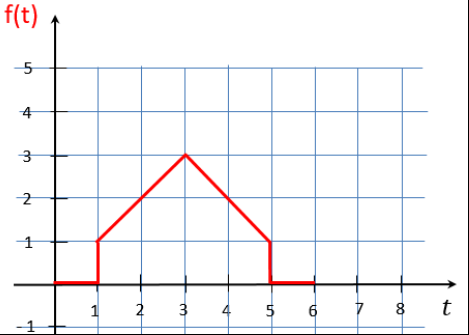
\includegraphics{zeitfunktion2.png}\\
  a) Bestimmen Sie $f(t)$! 3
  b) Bestimmen Sie die Laplace-Transformierte $F(s) = L{f(t)}$!
  c) Durch periodische Fortsetzung von $f(t)$ in $t=6$ entsteht die Funktion $f_p(t)$. (siehe Grafik)\\
  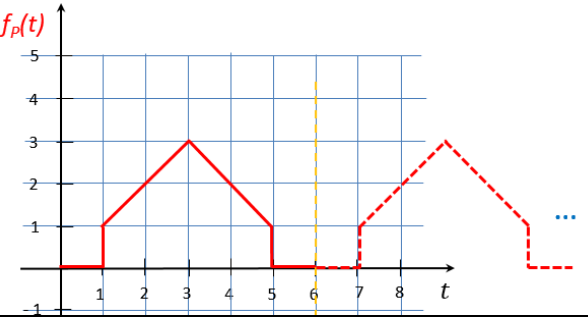
\includegraphics{zeitfunktion2a.png}\\
  Bestimmen Sie die LaplaceTransformierte $F_p(s) = L{f_p(t)}$!\\
  d) Existiert die Fouriertransformierte zu f(t) (Begründung erforderlich!)?\\
  e) $f(t)$ wird nun auch für negative Zeiten in $t=6$ periodisch fortgesetzt, daraus entsteht die Funktion $f_2p(t)$.\\
  Bei welchen Kreisfrequenzen hat die Fouriertransformierte $F_{2p}(\omega)$ = $F{f_{2p}(t)}$ von Null verschiedene Werte?\\
  \newpage
  Gegeben sei die folgende Schaltung:\\
  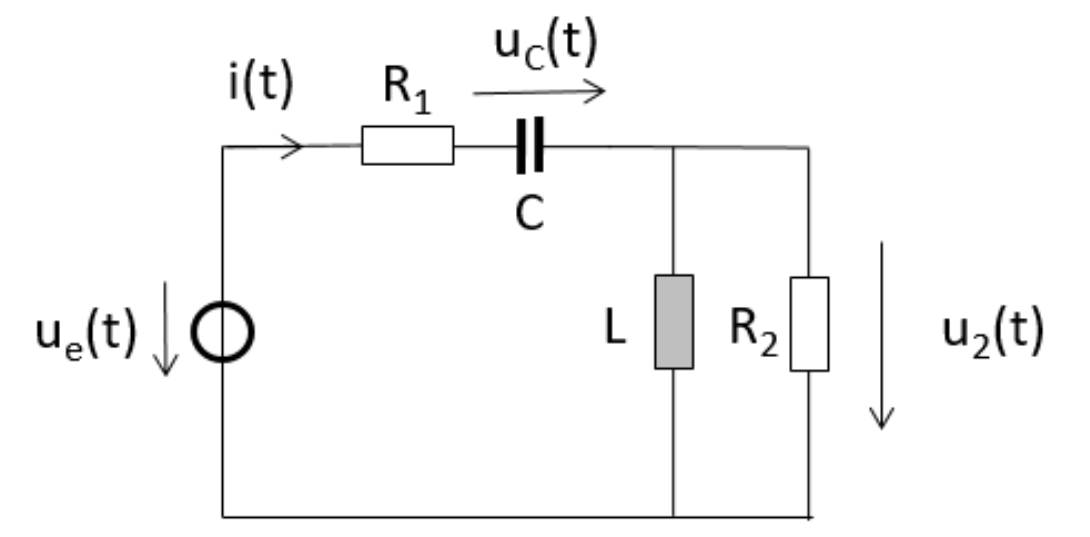
\includegraphics{Schaltung2.png}\\
  a) Bestimmen Sie die Übertragungsfunktion $G(s) = U_2(s)U_e(s)$!\\
  b) Die Anfangswerte $i_L(-0)= i_{L0} und u_C(-0) = u_{C0}$ sind nun von Null verschieden sind!\\
  Soll weiter die Operatorenmethode angewendet werden, muss die Schaltung erweitert werden. Zeichnen sie die erweiterte Schaltung!\\
  Gegeben ist die Übertragungsfunktion $G(s)= \frac{10}{s^2+2s+10}$\\
  c)Ist das System stabil (Begründung erforderlich)!\\
  d) Berechnen Sie den Endwert von $h(t)$!\\
  e) Mit welchem zeitlichen Übergangsverhalten müssen sie rechnen?\\
  \newpage
  Die Differentialgleichung eines Systems lautet:$y'''(t) + y''(t) - 2y'(t) = e^{-t}$
  mit den Anfangswerten $y(-0) = 1$, $y'(-0) = -2$ und $y(0)''(-0) = 3$\\
  a) Berechnen sie $y(t)$ mit Hilfe der Laplace-Transformation\\
  \newpage
  Gegeben ist die folgende Zeitfunktion $f(t) =\frac{t^2}{T^2}$ im Intervall 0 bis T. Die Funktion wird periodisch fortgesetzt.\\
  a) Bestimmen Sie den komplexen Fourierkoeffizienten $c_0$ der zugehörigen Fourierreihe!\\
  b) Bestimmen Sie für diese Reihe den allgemeinen komplexen Fourierkoeffizienten $c_k$ für $k\neq 0$ und stellen ihn so einfach wie möglich dar.
  \newpage
  Gegeben ist die Übertragungsfunktion einer elektrischen Schaltung: $G(s) = \frac{s}{s^2+2s+1}$\\
  a) Bestimmen Sie das Ausgangssignal (normierter Strom $i(t)$) für das folgende Eingangssignal (normierte Spannung $u(t)$):\\
  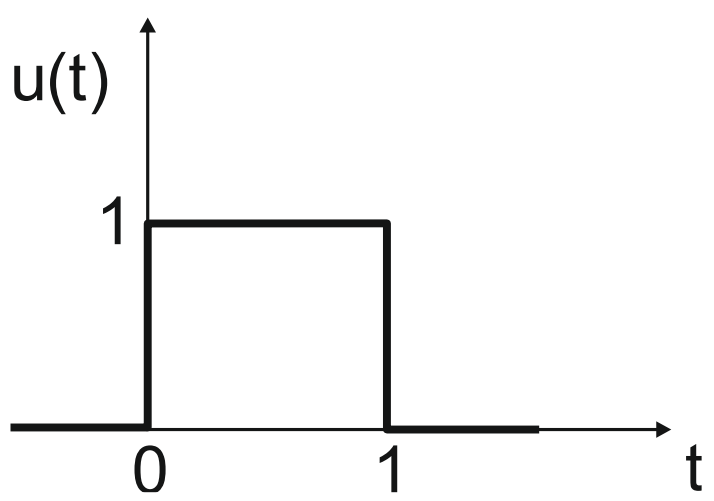
\includegraphics{zeitfunktion3.png}\\
  b) Bestimmen Sie i(t) für t gegen unendlich.\\
  c) Zeichnen Sie eine elektrische Schaltung, die die obige Übertragungsfunktion erfüllt und geben Sie die normierten Bauelementwerte an.\\
  \newpage
  Gegeben sei die Zeitfunktion f(t):\\
  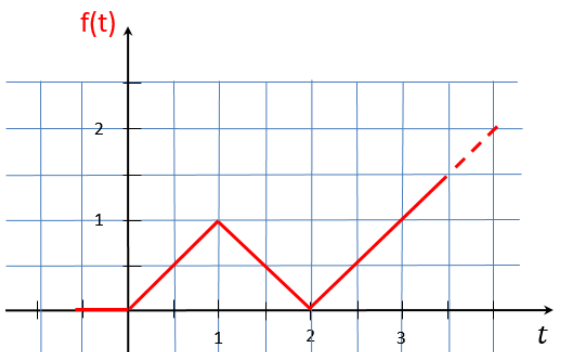
\includegraphics{zeitfunktion4.png}\\
  Bestimmen Sie f(t)!\\
  Handelt es sich bei f(t) um ein Leistungssignal? (Begründung erforderlich)!\\
  Bestimmen Sie die Laplace-Transformierte $F(s) = L{f(t)}$!\\
  Gegeben ist Laplace-Transformierte $M(s) = \frac{(1-e^{-s})s+e^{-s}}{s^2}$. Berechnen Sie die zugehörige kausale Zeitfunktion m(t)!\\
  \newpage
  Gegeben sei folgende Schaltung:\\
  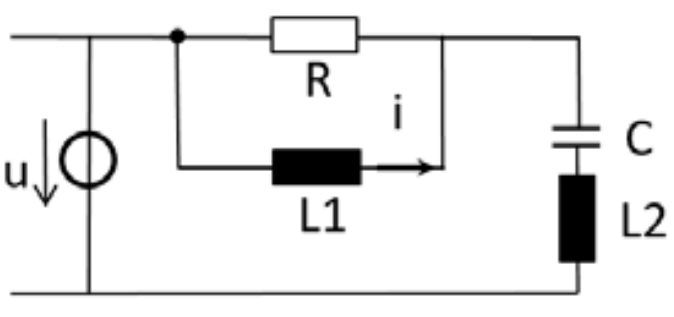
\includegraphics{Schaltung3.png}\\
  Bestimmen Sie die Übertragungsfunktion $G(s) = \frac{I(s)}{U(s)}$\\
  Im Weiteren sei die Übertragungsfunktion $G(s) = \frac{s+3}{(s+2)(s+1)^2}$!\\
  b) Ist das System mit dieser Übertragungsfunktion stabil (Begründungerforderlich)?\\
  c) Skizzieren Sie $h(t)$! (Anfangs- und Endwert, Einschwingzeit,Übergangsverhalten)!\\
  d) Die Eingangsgröße u(t) zeigt folgende Skizze. Berechnen Sie U(s)! \\
  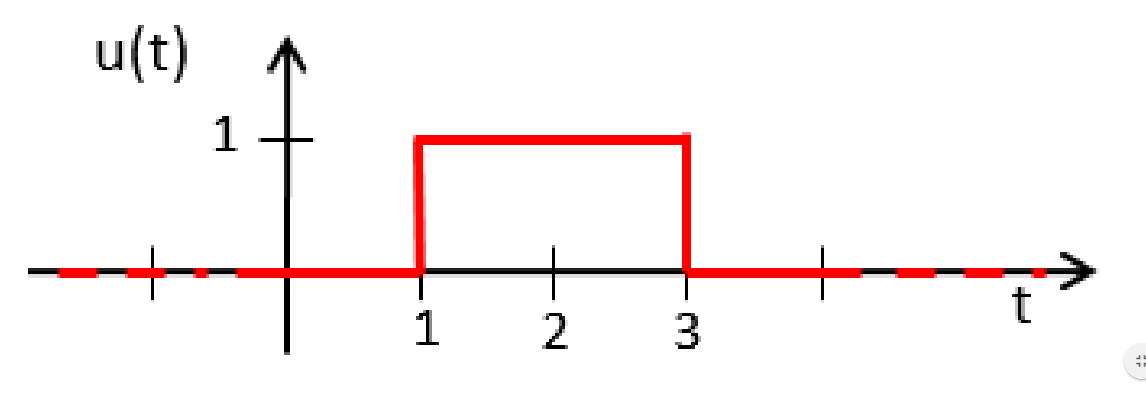
\includegraphics{zeitfunktion5.png}\\
  e) Berechnen Sie den Ausgang $v(t)$ des Systems mit der Eingangsgröße aus d)\\
  \newpage
  Ein PWM-Signal der Periodendauer T hat eine Impulslänge a<T (s.Skizze).\\
  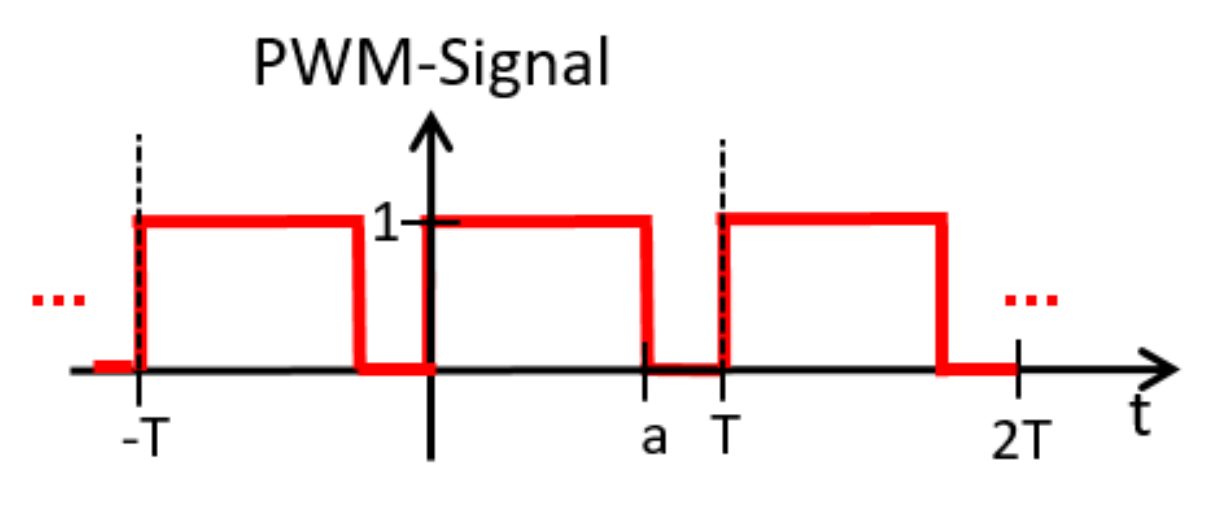
\includegraphics{zeitfunktion6.png}\\
  a) Berechnen Sie den komplexen Fourierkoeffizienten $C_0$ in Abhängigkeit von a!\\
  b) Berechnen Sie den allgemeinen Fourierkoeffizienten $C_k$ in Abhängigkeit von a!\\
  c) Berechnen Sie die Fouriertransformierte der Grundperiode\\
  d) Berechnen Sie die Fouriertransformierte des gesamten PWM-Signals!\\
  \newpage


  \addsec{Z-Trafo/Disktrete Systeme}
  Ein diskretes System hat die Differenzengleichung : $v_k - 0,6v_{k-1}+0,08v_{k-2}=u_{k-1}-0,1u_{k-3}$\\
  a) Geben Sie die Ordnung $n$ und die Diskrete Totzeit $dT$ des Systems an!\\
  b) Bestimmen Sie die Übertragungsfunktion $G(z)$ des Systems!\\
  c) Ist das System stabil? Begründen Sie Ihre Antwort!\\
  d) Im Schritt $k=0$ wird der Eingang $ \sigma[k]$ aufgeschaltet. Die Vergangenheitswerte sind $u_{-1} = u_{-2} = u_{-3} = 0$ und $v_{-1} = 0, v_{-2} = -1$\\
  Berechnen Sie den Ausgang $V(z)$!\\
  e) Berechnen Sie mit dem Ergebnis aus d) den Ausgang v[k]!\\
  \newpage

  Gegeben ist die Z-Übertragungsfunktion eines Systems: $G(z) = \frac{0,5z^2 - 0,5z+ 1}{z^2}$\\
  a) Bestimmen und skizzieren Sie die Impulsanwort $g[k]$.\\
  b) Bestimmen und skizzieren Sie die Sprungantwort $h[k]$ im Bereich von $k=-2$ bis $k=4$.\\
  Gegeben ist: $G(z) = \frac{z+1}{z^2 -2,5z +1}$\\
  c) Bestimmen Sie g[k].\\
  d) Ist das System stabil? Begründen Sie Ihre Antwort\\
  \newpage

  Ein diskretes System hat die Übertragungsfunktion: $G(z) = \frac{z+0,5}{(z-0,8)(z-0,2)}$\\
  a) Geben Sie die Differenzengleichung des Systems an!\\
  b) Berechnen Sie allgemein die Übergangsfolge h[k] des Systems! \\
  c) Berechnen Sie die ersten 4 Werte der Gewichtsfolge g[k] des Systems! \\

\end{document}